\chapter{Bose-Einstein Kondensation\label{chapter:bose}}
\lhead{Bose-Einstein Kondensation}
\begin{refsection}
\chapterauthor{Reto Christen und Daniel Gubser}

\section{Einleitung}
1924 erkannte der indische Physiker Satyendranath Bose\index{Bose, Satyendranath}, dass es bei ganz tiefen Temperaturen einen noch unbekannten quantenmechanischen Aggregatszustand gibt, welcher spezielle Eigenschaften besitzt. Er teilte diese Erkenntnis mit Albert Einstein, \index{Einstein, Albert} welcher die Wichtigkeit dieser Erkenntnisse erkannte. Weitere Berechnungen von Albert Einstein ergaben, dass dieses sogenannte Bose-Einstein-Kondensat (BEC)\index{Bose-Einstein-Condensat, BEC} zwar m"oglich sei, dazu m"ussten allerdings Temperaturen knapp "uber dem absolutem Nullpunkt erreicht werden, welches dazumal als unm"oglich galt. 

1938 konnte Helium auf $2.17~K$ abgek"uhlt werden und erreichte somit die Suprafluidit"at\index{Suprafluidit\"at}. Dieses Ph"anomen zeichnet sich dadurch aus, dass Helium die innere Reibung verliert und somit an Gef"assw"anden aufw"arts fliessen kann. Dieser Effekt war zwar noch keine Bose-Einstein-Kondensat, es kam dem jedoch bereits etwas n"aher. \cite{bose:WikiSuprafluid}

Erst durch die wesentlichen Verbesserungen der Abk"uhlungstechniken konnte im Jahre 1995 das erste Bose-Einstein-Kondensat erzeugt werden. Daf"ur wurde den Physikern Wolfgang Ketterle\index{Ketterle, Wolfgang}, Eric Cornell\index{Cornell, Eric} und Carl Wieman\index{Wieman, Carl} im Jahre 2001 den Nobel Preis verliehen. 

\begin{figure}
	\centering
	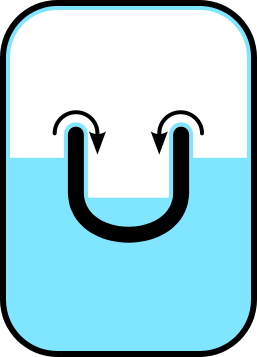
\includegraphics[width = 0.2\textwidth]{./bose/helium.png} 
	\caption[Suprafluides Helium]{Suprafluides Helium \cite{bose:WikiSuprafluid}}
	\label{fig:Helium}
\end{figure}

\section{Grundlagen}

Um ein Bose-Einstein-Kondensat zu erzeugen, sind Temperaturen nah dem Nullpunkt n"otig. Ausserdem k"onnen nur bestimmte Teilchen ein solches Kondensat bilden.

\subsection{Bosonen}

Die wichtigsten Eigenschaften von Bosonen nochmals kurz zusammengefasst.

\begin{itemize}
    \item	Bosonen sind die Elementarteilchen, welche gew"ohnlich f"ur die
            "Ubertragung von Kr"aften zust"andig sind.	 
    \item	Alle Bosonen haben einen ganzzahligen Spin. Sie unterliegen
            somit nicht dem Pauli-Prinzip.
    \item	Dies bedeutet, dass viele Bosonen denselben
            quantenmechanische Zustand besiedeln k"onnen.
\end{itemize}

\subsection{Abk"uhlung}

Um die tiefen Temperaturen erreichen zu k"onnen, werden zuerst mit Lasern die Atome abgek"uhlt und anschliessend mittels evaporativer K"uhlung die Zieltemperatur erreicht. 

Im Bild \ref{fig:LaserKuehlung} ist schematisch der Aufbau der Laserk"uhlung\index{Laserk\"uhlung} dargestellt.
Falls sich ein Atom bewegt, wird es mit dem Laser beschossen. Sobald Atom und Photon aufeinander treffen, wird Impuls ausgetauscht und dadurch das Atom abgebremst.
Da die Bewegung eines Atoms ein Mass f"ur seine Energie oder auch Temperatur ist, k"onnen mithilfe der Laser die Atome bis zu einigen $100~\mu K$  abgek"uhlt werden. \cite{bose:LaserKuehlung}

\begin{figure}
	\centering
	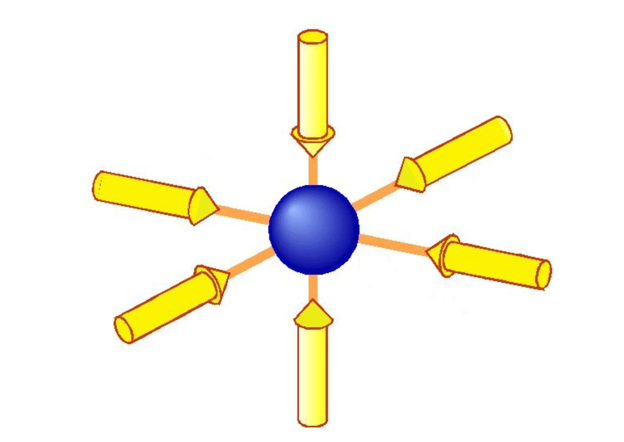
\includegraphics[width = 0.5\textwidth]{./bose/laserkuehlung.png} 
	\caption[Laserk"uhlung]{Laserk"uhlung \cite{bose:WikiLaserKuehl}}
	\label{fig:LaserKuehlung}
\end{figure}

Um die Atome nun noch weiter abk"uhlen zu k"onnen, wird die evaporative K"uhlung\index{Evaporative K\"uhlung} angewendet. Dieses Prinzip kann sehr gut mit einer heissen Tasse Kaffee veranschaulicht werden, wie dies in Abbildung \ref{fig:EvaporativeKuehlung} dargestellt ist. Die schnellen Atome haben eine hohe Temperatur und k"onnen beim ''Anhauchen'' der Tasse diese verlassen. Die langsameren und k"alteren Atome bleiben in der Tasse zur"uck.

Umgesetzt wird die ''Tasse'' durch Magnetfelder, somit entsteht eine Falle in der sich die Atome befinden. Die St"arke des Magnetfeldes bestimmt dabei welche Energien eingeschlossen werden k"onnen, langsame Atome bleiben in der Falle. Durch sukzessive Abschw"achung des Magnetfeldes, im Falle der Tasse eine Verkleinerung des Randes, verlassen immer mehr Teile das Magnetfeld und die Gesamttemperatur wird dadurch geringer. Schlussendlich beinhaltet das Magnetfeld nur noch wenige Teilchen, welche sich sehr nahe am absoluten Nullpunkt befinden. In aktuellen Experimenten am MIT\index{MIT} sind dies Temperaturen um $177~nK$, was "uber einer Million Mal k"alter als im Weltall ist. \cite{bose:WikiEvaporativeKuehlung}

\begin{figure}
	\centering
	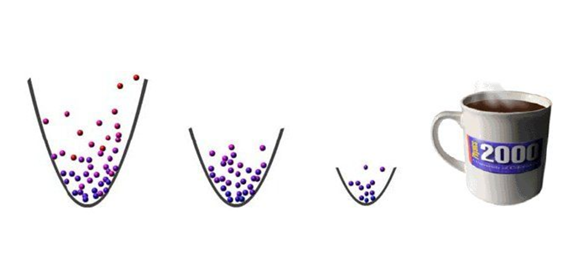
\includegraphics[width = 0.5\textwidth]{./bose/evaporation.png}
	\caption{Evaporative K"uhlung mit einer Tasse dargestellt.}
	\label{fig:EvaporativeKuehlung}
\end{figure}

\subsection{Eigenschaften}
Ein Bose-Einstein-Kondensat besteht aus Bosonen\index{Bosonen}, welche nahe auf den absoluten Nullpunkt heruntergek"uhlt werden. Dabei m"ussen Temperaturen unter $1~uK$ erreicht werden.
 
Bosonen haben die Eigenschaft, dass ihrer Spin immer ganzzahlig ist. Dies kann auch mit zwei wechselwirkenden Teilchen mit je einem Spin von $+1/2$ oder $-1/2$ erreicht werden. Solche Verbindungen sind unter anderem Cooper-Paare, welche im Kapitel \ref{chapter:supraleitung} genauer erl"autert werden. 

Eine weitere M"oglichkeit besteht darin, Elemente zu verwenden, welche bereits aus Bosonen bestehen. Das wichtigste Element in dieser Kategorie ist das Helium-4. Es besteht aus je zwei Protonen, Neutronen und Elektronen und verh"alt sich somit wie ein Boson. Am MIT werden aktuell Natrium-23 und Rubidium-87 verwendet. Beide Isotope bestehen wie das Helium-4 aus Bosonen und besitzen somit einen ganzzahligen Spin.

Werden diese Bosonen nun stark abgek"uhlt, bilden sie eine Einheit, sprich sie ''verschmieren'' zu einer gemeinsamer Wellenfunktion. Somit verhalten sich alle Teilchen im Bose-Einstein-Kondensat identisch und sind ununterscheidbar.

\subsection{Effekte}

Durch diese Koh"arenz\index{Koh\"arenz} und Ununterscheidbarkeit der einzelnen Teile resultieren diverse Effekte wie die Suprafluidit"at\index{Suprafluidit\"at} oder Supraleitung\index{Supraleitung}. Das Bose-Einstein-Kondensat ist f"ur diese Effekte zwar nicht die einzige Erkl"arung, hat aber einen wichtigen Einfluss darauf. 

Ebenfalls ergaben sich bei der Herstellung von Bose-Einstein-Kondensat weitere interessante Effekte, welche f"ur diverse Anwendungen genutzt werden k"onnen. Dies ist zum Beispiel die Erkl"arung, wie Neutronensterne\index{Neutronensterne} aufgebaut sind oder der Big Bang\index{Big Bang} entstand. Durch die absolute Koh"arenz k"onnen auch neue Laser\index{Laser} entwickelt werden, sogenannte Atom-Laser\index{Atom-Laser}. Diese Atom-Laser k"onnen im Quantencomputer\index{Quantencomputer} Bereich neue Fortschritte mit sich bringen sowie auch bei Quanten-Teleportation. Ein weiterer wichtiger Effekt ist das Abbremsen von Licht ohne dabei an Impuls zu verlieren.


\section{Mathematischer Hintergrund}

Grunds"atzlich werden in diesem Teil die gleichen Berechnungen wie im Buch von Richard P. Feynman\index{Feynman, Richard P.} \cite{bose:feynman} verwendet. F"ur die bessere Verst"andlichkeit werden die Formel, im Gegensatz zum Buch, etwas genauer erl"autert.

Als Ausgangslage dient ein geschlossenes System aus Teilchen, welches mit einem Teilchenreservoir verbunden ist. 
Zwischen dem System und dem Reservoir k"onnen Teilchen ausgetauscht werden. Dies ist in Abbildung \ref{fig:reservoir} dargestellt.

\begin{figure}
	\centering
	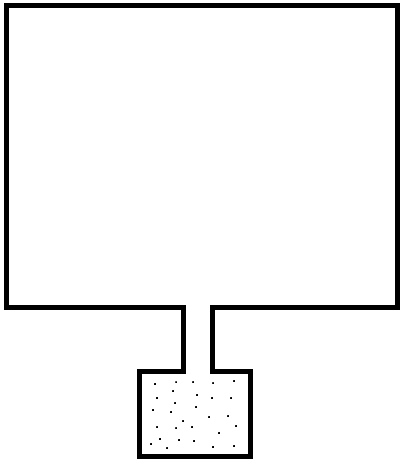
\includegraphics[width = 0.4\textwidth]{./bose/reservoir.png}
	\caption{Reservoir}
	\label{fig:reservoir}
\end{figure}
Die Energie eines Teilchens berechnet sich nach der Formel:

\begin{equation}
   E_n = \frac{p^2}{2m}
\end{equation}
Die Wahrscheinlichkeit, mit der diese Energie im System zu finden ist, l"asst sich mit der folgender Formel berechnen.

\begin{equation}
    P(E_n) = \frac{e^{-E_n/kT}}{\sum\limits_{n = 1}^{N} e^{-E_n/kT}}    
\end{equation}
Der Nenner stellt dabei die Verteilung der Energien dar. Um den Ausdruck etwas kompakter zu formulieren wird $ \beta = \frac{1}{kT}$ eingef"uhrt.

\begin{equation}
    Q = \sum\limits_{n = 1}^{N} e^{-E_n/kT} = \sum\limits_{n = 1}^{N} e^{-\beta E_n}
\end{equation}

Die mittlere Energie des Systems betr"agt:
\begin{equation}
    \langle U \rangle = \sum_{n} E_n \cdot P(E_n) = \sum_{n} E_n \cdot \frac{e^{-\beta E_n}}{Q}
\end{equation}
Durch Ableiten der eulerschen Funktion nach $\beta$ kann die Formel weiter vereinfacht werden. Beim Ableiten wird die Energie $E_n$ als Faktor entstehen.

\begin{equation*}
\langle U \rangle = \sum_{n} E_n \cdot \frac{e^{-\beta E_n}}{Q} = -\frac{1}{Q} \sum_{n} \frac{d}{d \beta} e^{-\beta E_n} 
\end{equation*}
Die Ableitung nach $\beta$ kann vor der Summe durchgef"uhrt werden, dadurch erh"alt man die Definition von $Q$.
\begin{equation*}
\langle U \rangle = -\frac{1}{Q} \frac{d}{d \beta} \sum_{n}  e^{-\beta E_n}  = -\frac{1}{Q} \frac{d}{d \beta}Q
\end{equation*}
In dieser Formel ist $Q$ zweimal vorhanden, einmal im Bruch und einmal abgeleitet. Dieser Term kann auch auf andere Art und Weise geschrieben werden, n"amlich mit der Ableitung des Logarithmus von $Q$. Damit erh"alt man eine sehr kompakte Darstellung der mittleren Energie.
\begin{equation}
\langle U \rangle = -\frac{d}{d \beta} ln(Q)
\end{equation}

Nun werden einige Umformungen durchgef"uhrt um das Berechnen der Gesamtenergie des Systems zu vereinfachen.
Als erstes wird angenommen, dass nur ein einziger Energiezustand existiert.
Dadurch kann man eine Klammer mit Summanden ausschreiben, in Rot dargestellt.
Kommen nun weitere Energiezust"ande hinzu, blaue Klammern, so k"onnen diese Klammern miteinander multipliziert werden.
Dies f"uhrt dazu, dass das Produktzeichen f"ur die Zust"ande verwenden k"onnen.


\begin{equation}
Q = \sum\limits_{n_0, n_1,...} e^{- \beta \sum_a \epsilon_a n_a } 
=  \sum^N  \textcolor{red}{ e^{- \beta \epsilon_0 n_0 }} \textcolor{blue} {e^{- \beta \epsilon_1 n_1 }} e^{- \beta \epsilon_2 n_2 } ... 
\end{equation}

\begin{equation*}
= \textcolor{red} {(1+e^{- \beta \epsilon_1 }+e^{- \beta \epsilon_2*2  }+e^{- \beta \epsilon_3*3  }+...)} \cdot \textcolor{blue} {(1+e^{- \beta \epsilon_1 }+e^{- \beta \epsilon_1*2  }+e^{- \beta \epsilon_1*3  }+...)} \cdot ...
\end{equation*}

\begin{equation}
\sum\limits_{n_0, n_1,...} e^{- \beta \sum_a \epsilon_a n_a } = \prod_{a} \sum_{n_i} e^{- \beta \epsilon_a n_i }
\end{equation}
Die Summe stellt die geometrische Reihe dar, dadurch kann die ganze Summe durch einen simplen Bruch ersetzt werden. Substitution der e-Funktion mit $q$ und $n_i$ mit $i$.

\begin{equation}
\sum_{n_i} (e^{- \beta \epsilon_i })^{n_i} = \sum_{i} q^i = \frac {1}{1-q}
\end{equation}
Angewendet ergibt sich damit:

\begin{equation}
    \prod_{a} \sum_{n_i} e^{- \beta \epsilon_a n_i } = \prod_{a} \frac {1}{1-e^{- \beta \epsilon_a}}
\end{equation}
Das Produkt kann durch Anwendung der Logarithmen Regeln in eine Summe umgeformt werden.

\begin{equation}
\ln \left[ \left( \frac{1}{1-e^{\beta \epsilon_{a_0}}} \right) \cdot \left( \frac{1}{1-e^{ \beta \epsilon_{a_1}}} \right) \cdot ...\right] = \ln \left( \frac{1}{1-e^{\beta \epsilon_{a_0}}} \right) + \ln \left( \frac{1}{1-e^{\beta \epsilon_{a_1}}} \right) + ...
\end{equation}
Dies f"uhrt schliesslich zur Formel:

\begin{equation}
Q = \prod_{a} \frac {1}{1-e^{- \beta \epsilon_a}} = \sum_{a} \ln \left( 1-e^{- \beta \epsilon_a} \right)
\end{equation}
Damit Teilchen zwischen dem System und dem Reservoir ausgetauscht werden k"onnen, muss Energie aufgewendet werden.
Dies wird mit einem zus"atzlichen Term abgegolten. Damit wird $Q$ abh"angig von dieser Energie $\mu$.


 \begin{equation}
 Q^{(\mu)} = \sum e^{- \beta \sum_{a} (\epsilon_a - \mu)n_a} = e^{-\beta g}
 \end{equation}
umgeformt auf $g$

  \begin{equation}
  -\frac{1}{ \beta } \ln(Q^{\mu}) = g
  \end{equation}
Die Berechnung der Gesamtenergie wird durch folgende Annahme vereinfacht. 
Es wird angenommen, dass es sich nicht um diskrete sondern um kontinuierliche Energiezust"ande handelt.

\begin{equation}
\frac{1}{\beta} \sum_{a} \ln(1-e^{-\beta (\epsilon_a -\mu)}) \approx \frac{1}{\beta} \int \ln(1-e^{-\beta (\epsilon_a-\mu)})
\end{equation}
Damit Berechnet sich die Gesamtenergie des Systems.
Da die Teilchen sich in drei Dimensionen bewegen k"onnen, muss ein Dreifachintegral gel"ost werden.
Ausserdem findet sich im Integral der Term ''Wert mal Wahrscheinlichkeit'' im Bruch wieder, unser Q.

\begin{equation}
U = s \int  \frac{ \left(e^{ {\frac{- \beta p^2}{2m}} } e^{\beta \mu} \right) \cdot {\frac{p^2}{2m}} }{1-e^{ {\frac{- \beta p^2}{2m}} } e^{\beta \mu}} \cdot \frac{d^3 p}{(2 \pi \hbar)^3}
\end{equation}
Die Vereinfachung ist bis zu einer kritischen Temperatur zul"assig. Ab dieser Temperatur d"urfen die kleinsten Energien des Systems nicht mehr vernachl"assigt werden. F"ur sehr tiefe Temperaturen m"ussen die kleinen Terme ber"ucksichtigt werden. Berechnet man die Gesamtenergie des Systems numerisch, erh"alt man Resultate, welche nicht sinnvoll sind.

\begin{equation}
\frac{1}{\beta} \sum_{a} \ln(1-e^{-\beta (\epsilon_a-\mu)}) \neq \frac{1}{\beta} \int \ln(1-e^{-\beta (\epsilon_a-\mu)})
\end{equation}
Dies spiegelt sich bei der W"armekapazit"at wieder, die eine sehr starke Steigung bei eben dieser Temperatur aufweist. Ein Vergleich der W"armekapazit"at zwischen dem Bose-Einstein Gas und fl"ussigem Helium ist in Abbildung \ref{fig:WrmKap} dargestellt. Zu erkennen ist die starke Steigung bei der kritischen Temperatur.

\begin{figure}
    \centering
    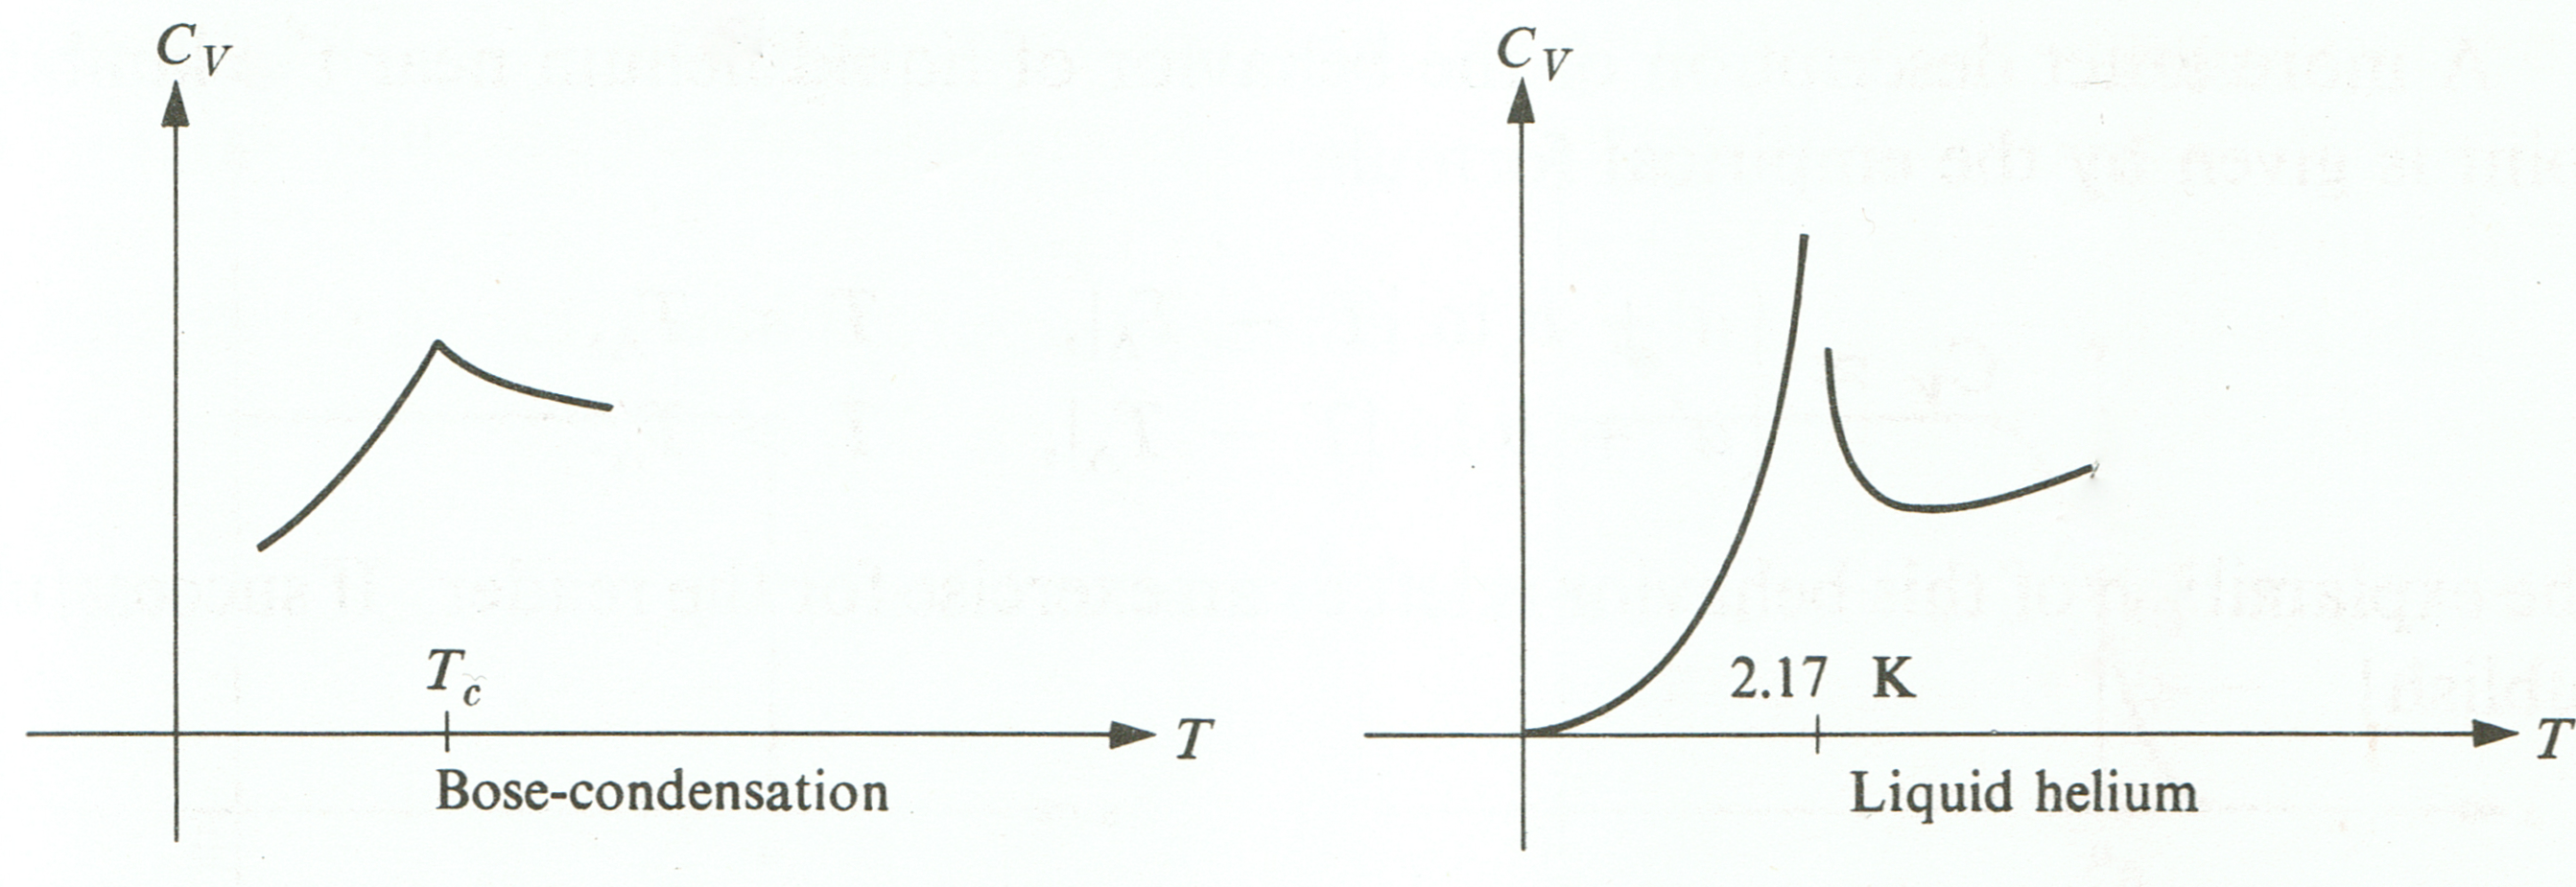
\includegraphics[width = 0.8\textwidth]{./bose/wrmkap.png}
    \caption[W"armekapazit"at eines Bose-Einstein Kondensats und fl"ussigem Helium.]{W"armekapazit"at eines Bose-Einstein Kondensats und fl"ussigem Helium. \cite{bose:feynman}}
    \label{fig:WrmKap}
\end{figure}
Wenn man sich die kontinuierliche Gaussverteilung eines Gases betrachtet, welches abgek"uhlt wird, verringert sich die Standardabweichung, welche die Temperatur darstellt.

\begin{figure}
    \centering
    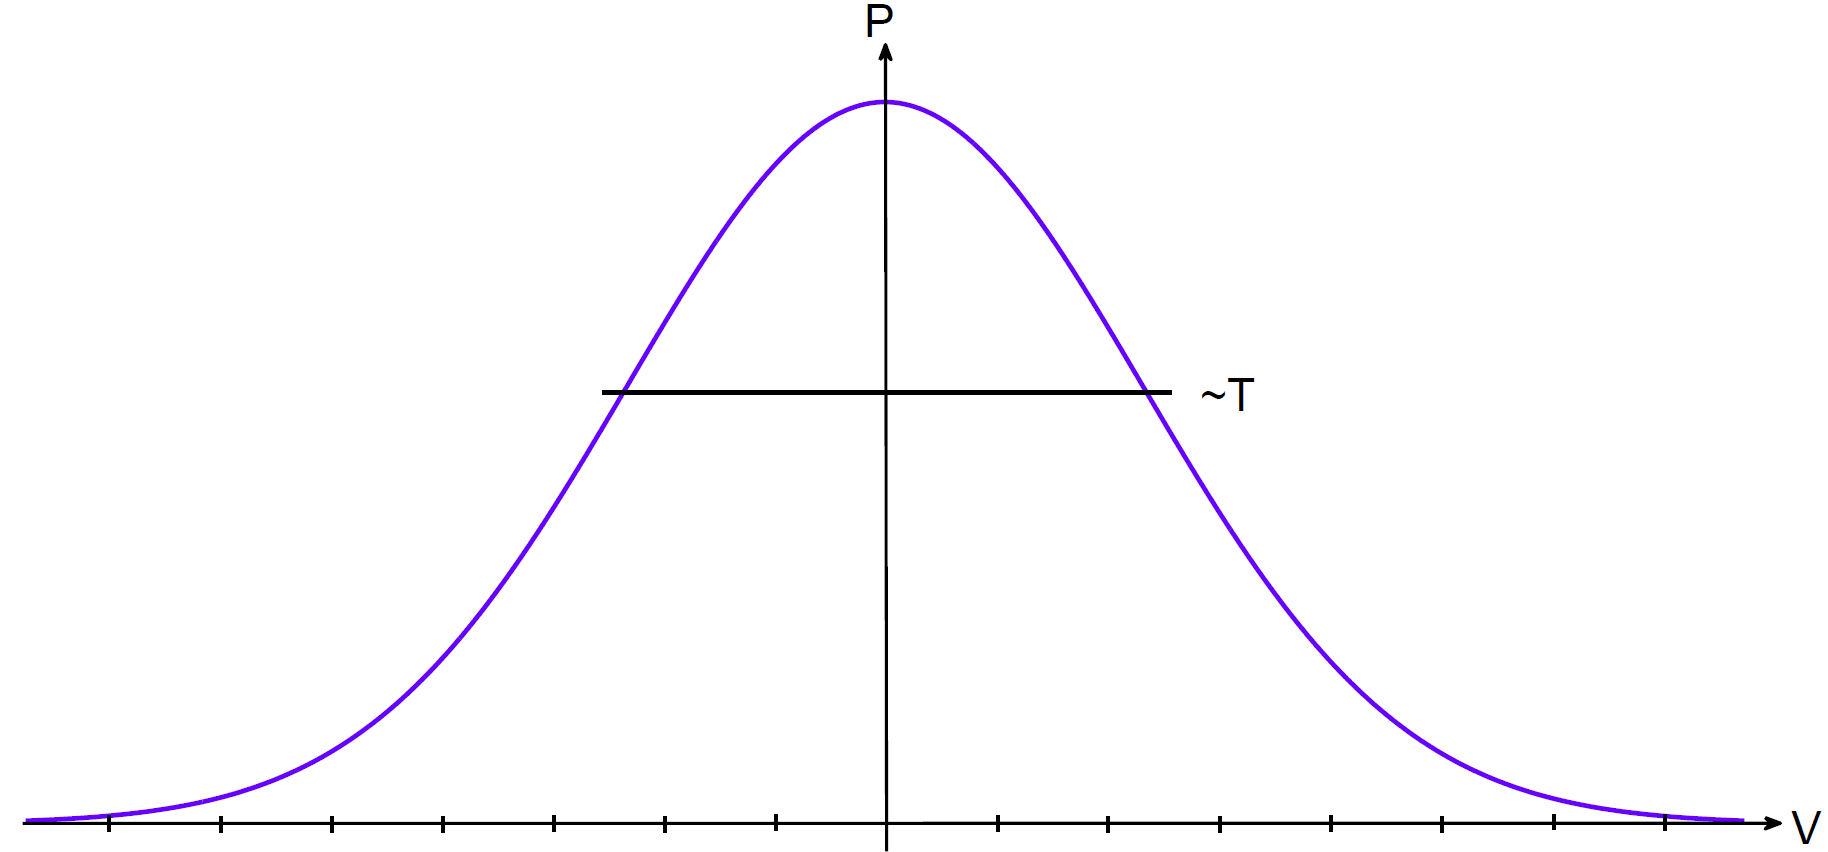
\includegraphics[width = 0.7\textwidth]{./bose/gauss1.png}
    \caption[Verteilung Ausgangstemperatur]{Verteilung zwischen Druck und Volumen eines Gases, Ausgangstemperatur.}
    \label{fig:Gauss1}
\end{figure}

\begin{figure}
    \centering
    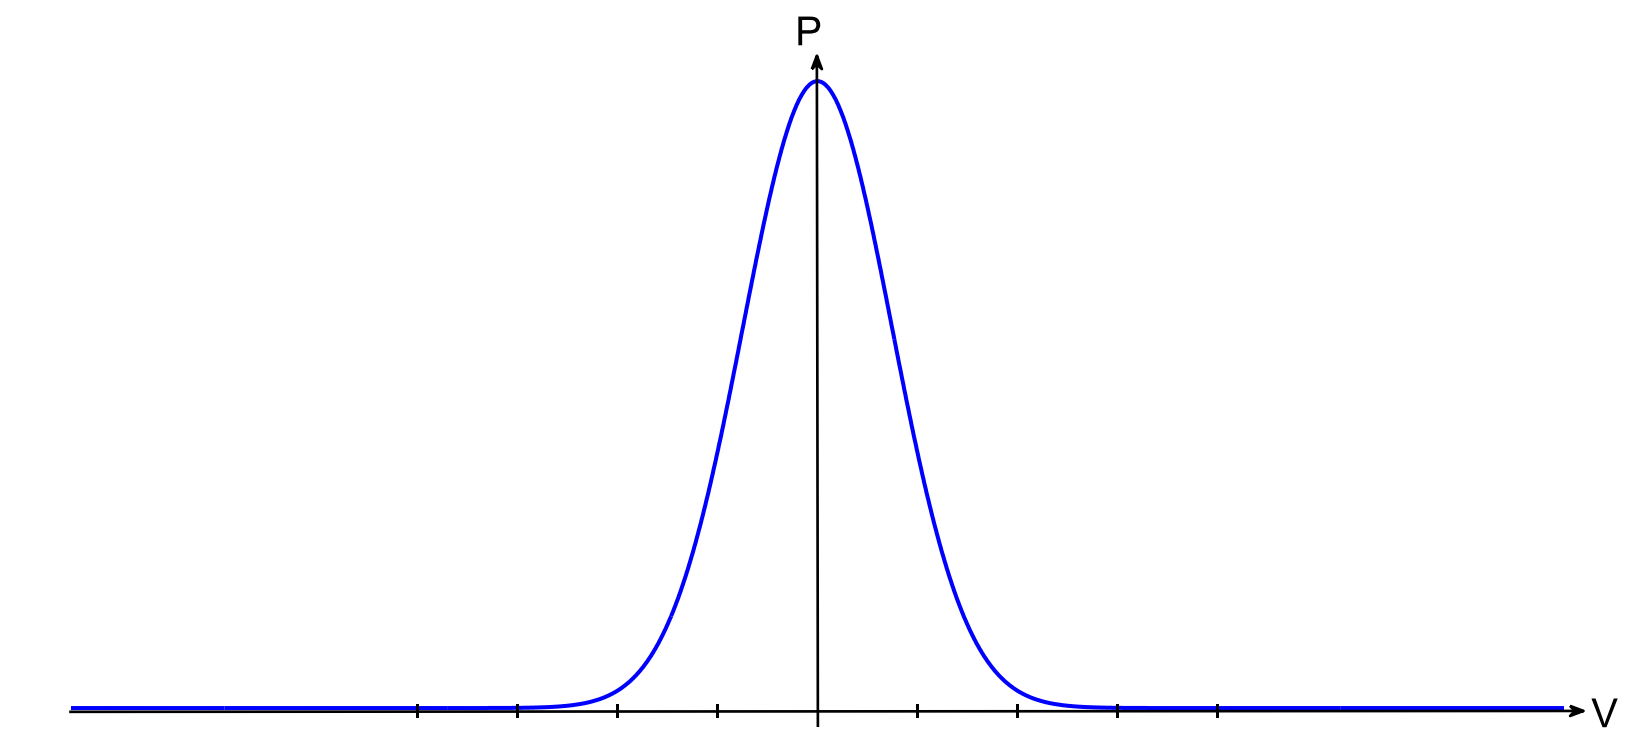
\includegraphics[width = 0.7\textwidth]{./bose/gauss2.png}
    \caption[Verteilung bei Abk"uhlung]{Verteilung zwischen Druck und Volumen eines Gases, bei Abk"uhlung. Die Standardabweichung wird geringer, damit auch die Temperatur.}
	\label{fig:Gauss2}
\end{figure}

\begin{figure}
    \centering
    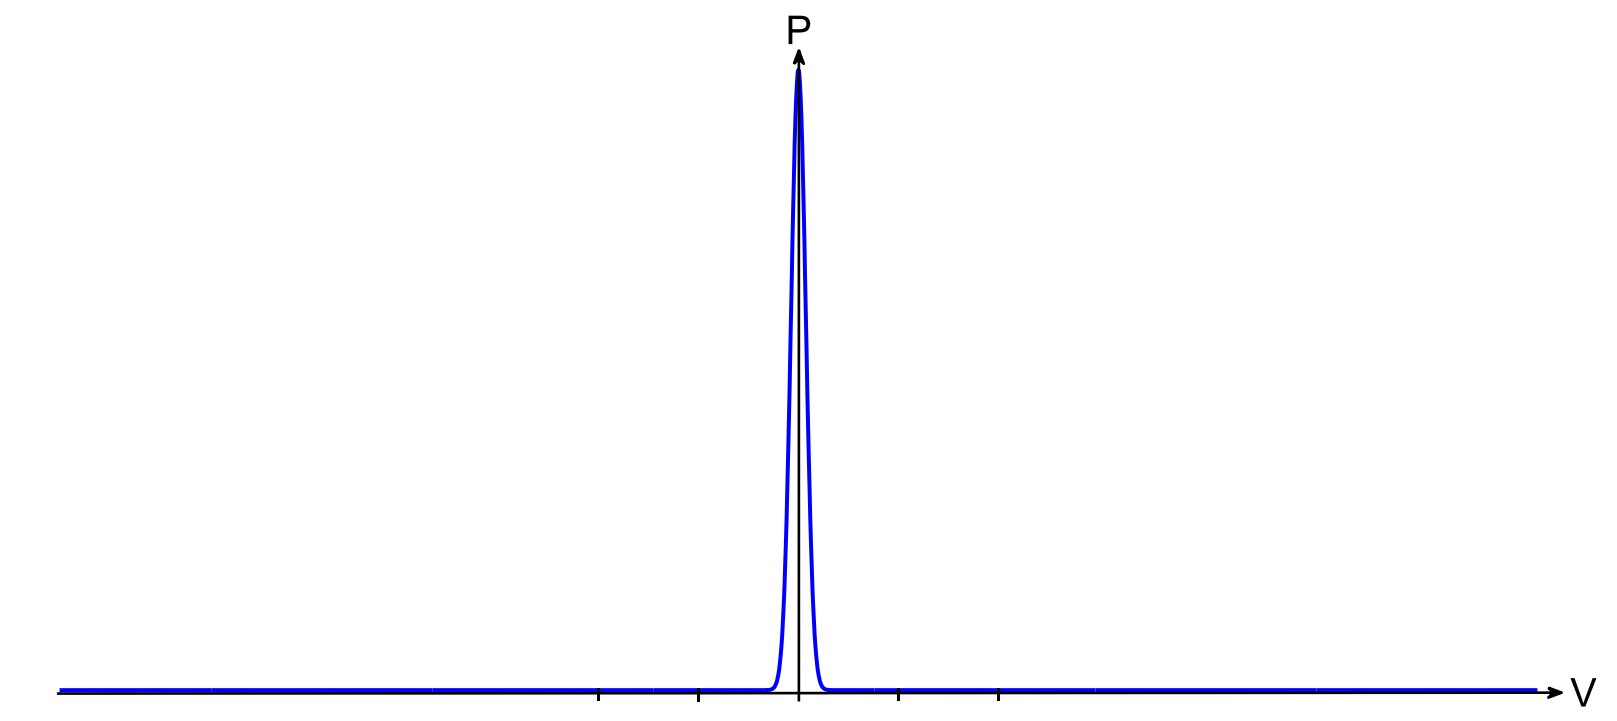
\includegraphics[width = 0.7\textwidth]{./bose/gauss3.png}
    \caption[Verteilung bei starker Abk"uhlung]{Verteilung zwischen Druck und Volumen eines Gases, bei starker Abk"uhlung. Die Standardabweichung wird noch geringer, damit auch die Temperatur.}
	\label{fig:Gauss3}
\end{figure}
F"ur das Bose-Einstein Kondensat liegt eine diskrete Verteilung vor.
Also wird eine Abk"uhlung dazu f"uhren, dass sich alle Teilchen in einen Zustand hin verschieben. Die x-Achse wurde unterteilt und soll die verschiedenen Energieniveaus darstellen, zuletzt kann nur noch ein Zustand eingenommen werden, n"amlich $v = 0$. 

\section{Anwendungen}
\subsection{Erkl"arung quantenphysikalischen Effekten}
Durch das Bose-Einstein-Kondensat k"onnen die Suprafluidit"at sowie die Supraleitung besser verstanden werden. Es ist zwar nicht der einzige Effekt der mitwirkt aber ein wichtiger. 

Supraleiter k"onnen in n"aher Zukunft eine wichtige Rolle in der Energieverteilung "ubernehmen. Kurze Leitungen, welche mit grosser Leistung belastet werden, stehen dabei im Vordergrund. Da ein Supraleiter weder einen Widerstand noch einen Skin-Effekt hat, k"onnen bei relativ kleinem Querschnitt grosse Str"ome "ubertragen werden. 
Aktuell ist eine $1~km$ lange Leitung in Essen in Betrieb genommen. Dies dient zwar als Versuchsaufbau, die Betreiberinnen erhoffen sich dabei aber wichtige Erkenntnisse, wie auch eine zuverl"assige Energieversorgung. \cite{bose:SupraVerteilnetze}

Ein Bose-Einstein-Kondensat kann ebenfalls zur Erkl"arung von Quark-Gluon-Plasma\index{Quark-Gluon-Plasma} beigezogen werden. Es wird angenommen, dass das Universum diesen Zustand des Quark-Gluon-Plasma Sekundenbruchteile nach dem Big Bang\index{Big Bang} durchlaufen hat. Ein Bose-Einstein-Kondensat verh"alt sich "ahnlich wie sehr heisse Atome unter grossem Druck. In beiden F"allen k"onnen sich die Wellen zu einer einzigen Wellenfunktion zusammenschliessen. Das einzige noch bestehende Quark-Gluon-Plasma wird in Neutronensternen vermutet. Dies konnte bis jetzt nicht bewiesen werden. \cite{bose:MITvideo}

\subsection{Atom-Laser}
Ein herk"ommlicher Laser nutzt die Koh"arenz von Photonen aus und erzeugt somit eine starke Lichtquelle. Werden nun aber Atome anstatt Photonen verwendet, liesse sich somit eine viel st"arkere Lichtquelle herstellen. Atome sind grunds"atzlich nicht koh"arent zu einander. Wird aber ein Bose-Einstein-Kondensat verwendet, in welchem alle Teile koh"arent zueinander sind, liesse sich ein Atom-Laser tats"achlich herstellen.

Mit einem Atom-Laser erg"aben sich grosse Fortschritte in der quantenmechanischer Teleportation sowie bei Pr"azisionsmessungen.

Gegenw"artig wird noch Grundlagenforschung betrieben. Einen funktionierenden Atomlaser wurde bereits 1997 von Wolfgang Ketterle realisiert, weil dieser jedoch nur f"ur kurze Impulse anwendbar ist, konnten keine Anwendungen damit erzielt werden. 

\subsection{Abbremsung von Photonen}

Ein weiterer Effekt ist die Abbremsung von Licht. In Versuchen mit einem Bose-Einstein-Kondensat zeigte sich, dass Licht effektiv abgebremst werden kann, ohne dass Informationen verloren gehen. Dies an sich ist nicht weiter verwunderlich, da die Lichtgeschwindigkeit in verschiedenen Medien variiert. Die Eigenartigkeit liegt in der Geschwindigkeit des Lichtes selber. In diversen Glase oder Diamanten kann eine Verlangsamung des Lichtes um den Faktor 2 - 3 beobachtet werden kann. Das Licht in einem Bose-Einstein-Kondensat wird aber bis auf $17~m/s$ abgebremst, was "uber hundert Millionen Mal langsamer ist. Warum dies so ist, kann bis jetzt nicht erkl"art werden. \cite{bose:SlowLight}

\section{Schlusswort}

Die Theorie der Bose-Einstein-Kondensation kann divers quantenmechanische Ph"anomene teilweise oder ganz erkl"aren und ist deswegen f"urs Verst"andnis des Universums essentiell. Die praktische Umsetzung des Kondensat ergaben nicht nur die erwarteten Effekte, sondern auch noch vollkommen unbekannte Ph"anomene. Deshalb kann davon ausgegangen werden, dass auch in der Zukunft weiterhin neue Effekte entdeckt und f"ur weitere Forschungen gebraucht werden kann. 

\printbibliography[heading=subbibliography]
\end{refsection}



